% chktex-file 44

\section{\large Ejercicio 2. Dependencia Lineal, Independencia Lineal y Conjuntos Generadores.}

Considerando el conjunto \textbf{\textit{S}}, se plantean las siguientes preguntas:
\begin{itemize}
    \item ¿Es el conjunto \textbf{\textit{S}} linealmente independiente o dependiente?
    \item ¿\textbf{\textit{S}} genera al espacio tridimensional $\mathbb{R}^3$?
\end{itemize}

\[
    \text{\textbf{\textit{S}}}=\left\{(3,0,0),(0,1,1),(1,0,0)\right\}
\]

\textbf{Dependencia lineal}
\[
    \alpha\begin{bmatrix}
        3 \\
        0 \\
        0 \\
    \end{bmatrix}
    \beta\begin{bmatrix}
        0 \\
        1 \\
        1 \\
    \end{bmatrix}
    \lambda\begin{bmatrix}
        1 \\
        0 \\
        0 \\
    \end{bmatrix}
\]

\[
    (\alpha3,\alpha0,\alpha0)+(\beta0,\beta1,\beta1)+(\lambda1,\lambda0,\lambda0)
\]


\[
    (\alpha3+\beta0+\lambda1,\alpha0+\beta1+\lambda0,\alpha1+\beta0+\lambda0)
\]

\[
    \begin{aligned}
        \left(
            \begin{array}{ccc|c}
                3 & 0 & 1 & 0 \\
                0 & 1 & 0 & 0 \\
                0 & 1 & 0 & 0 \\
            \end{array}
        \right)
        &\frac{f1}{3} \\ \\
        \left(
            \begin{array}{ccc|c}
                1 & 0 & \frac{1}{3} & 0 \\
                0 & 1 & 0 & 0 \\
                0 & 1 & 0 & 0 \\
            \end{array}
        \right)
        &f2-1f3 \\ \\
        \begin{aligned}
            f2-1f3
            &\begin{array}{ccc|c}
                0 & 1 & 0 & 0 \\
                0 & -1 & 0 & 0  \\
                \hline
                0 & 0 & 0 & 0 \\ 
            \end{array}
        \end{aligned} \\ \\
        \left(
            \begin{array}{ccc|c}
                1 & 0 & \frac{1}{3} & 0 \\
                \cmidrule{1-1} \multicolumn{1}{c|}{0} & 1 & 0 & 0 \\
                \cmidrule{2-2} 0 & \multicolumn{1}{c|}{0} & 0 & 0 \\
            \end{array}
        \right)
    \end{aligned}
\]

\[
    \alpha+\frac{1}{3}\lambda=0
\]
\[
    \alpha=-\frac{1}{3}\lambda
\]
\[
    \beta=0
\]
\begin{figure}[ht!]
    \centering
    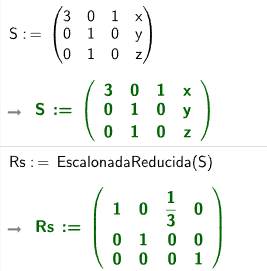
\includegraphics[width=150pt,height=200pt]{img/imagen10.png}
    \caption{Comprobación en GeoGebra}
\end{figure}
\begin{center}
    \textbf{Solución: }El conjunto de vectores \textbf{\textit{S}} es linealmente dependiente. Por tal motivo, este no es capaz generar el espacio tridimensional $\mathbb{R}^3$.
\end{center}
